\documentclass{beamer}

\usepackage[utf8]{inputenc}
\usepackage[T1]{fontenc}
\usepackage{graphicx}
\usepackage{hyperref}

\title{Image Embedding for Product Labeling}
\author{Couture Vision}
\date{\today}

\begin{document}

\frame{\titlepage}

\section{Project Objective}
\begin{frame}{Project Objective}

\textbf{Goal:}
\begin{itemize}
    \item Based on a photo of an article, match the reference image of this article.
\end{itemize}

\textbf{Example:}
\begin{columns}
    \column{0.5\textwidth}
    \begin{figure}[t]
        \includegraphics[width=\textwidth]{assets/shoes_test.jpg}
        \caption{Test Image}
    \end{figure}
    \column{0.5\textwidth}
    \begin{figure}[t]
        \includegraphics[width=\textwidth]{assets/shoes_reference.jpeg}
        \caption{Reference Image}
    \end{figure}
\end{columns}

\end{frame}

\begin{frame}{Dataset presentation}
    \begin{itemize}
        \item DAM : 2766 images = 2766 classes
        \item 80 test images without labels
        \item DAM images are clean : regular resolution and proper background
        \item test images : different resolutions, backgrounds; sometimes multiple items in one image.
        \item Basically no training set : we will focus on Siamese network methods : embedding images then comparing embeddings
        \item We (will) manually labelise the test dataset to have an accuracy.
    \end{itemize}
    \end{frame}
    
    \begin{frame}{Test images}
        \begin{figure}
            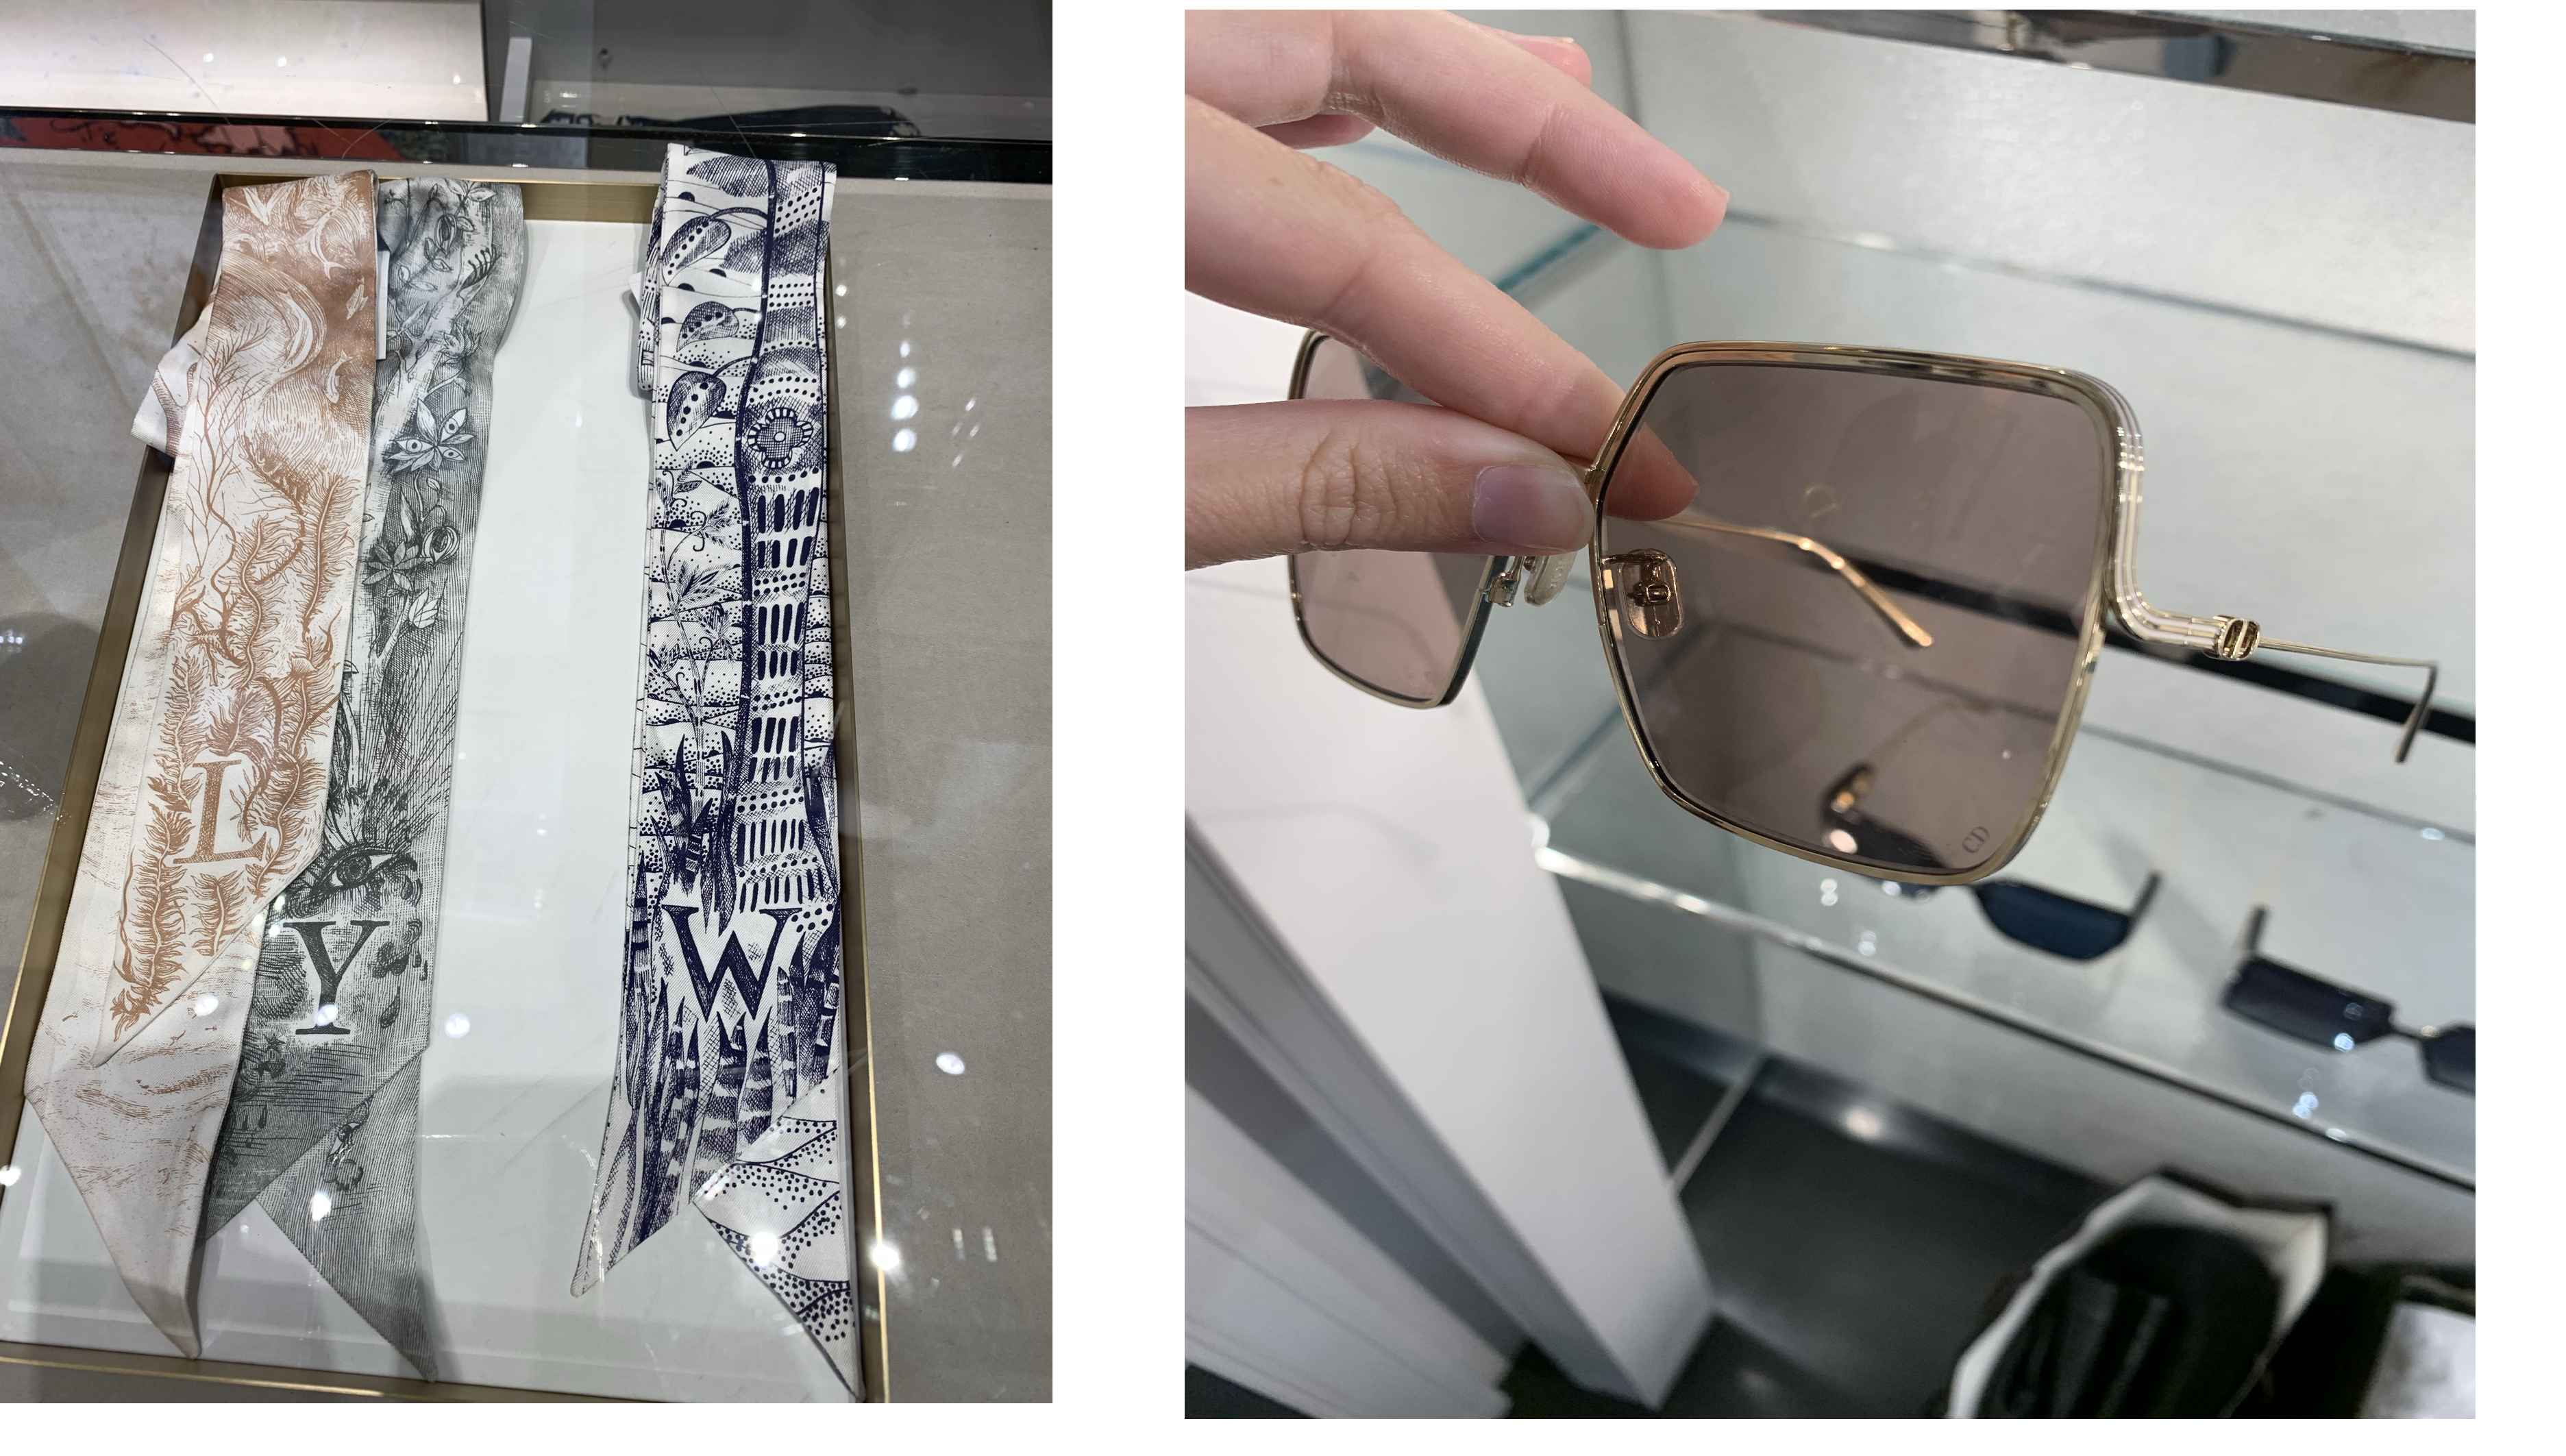
\includegraphics[width=\textwidth]{assets/p_img.png}
        \end{figure}
    \end{frame}

\section{Introduction}
\begin{frame}{Project Overview}
\begin{itemize}
    \item We utilized Microsoft's ResNet50 and Google's ViT to extract embeddings.
    \item Cosine similarity is used to find the best matches between images.
    \item We preprocess images using \texttt{rembg} to remove backgrounds, as test images (shop pictures) differ from the clean DAM images.
    \item Embedding extraction assists in labeling products by suggesting potential matches.
\end{itemize}
\end{frame}


\section{Methodology}
\begin{frame}{Embedding Extraction Pipeline}
\begin{columns}
    \column{0.5\textwidth}
    \begin{itemize}
        \item Use ResNet50 and ViT to extract image embeddings.
        \item Employ cosine similarity to rank matches.
        \item Preprocess test images with \texttt{rembg} to isolate objects from noisy backgrounds.
    \end{itemize}
    \column{0.5\textwidth}
    \begin{figure}
        \includegraphics[width=0.6\textwidth]{assets/pipeline_overview.png}
        \caption{Pipeline overview}
    \end{figure}
\end{columns}
\end{frame}

\begin{frame}{Embedding Extraction Pipeline}
    \begin{figure}
        \includegraphics[width=\textwidth]{assets/background_removal.png}
        \caption{Background removal using \texttt{rembg}, scaling and center-cropping}
    \end{figure}
\end{frame}

\begin{frame}{Good Classification Example}
\begin{itemize}
    \item Original image and extracted object.
    \item Top 5 matches with high similarity scores.
\end{itemize}
\begin{figure}
    \includegraphics[width=\textwidth]{assets/good_classification.png}
    \caption{Example of a good classification result}
\end{figure}
\end{frame}

\begin{frame}{Bad Classification Example}
\begin{itemize}
    \item Challenges: reflections on the glass adversely affecting background removal and embeddings.
\end{itemize}
\begin{figure}
    \includegraphics[width=\textwidth]{assets/bad_classification.png}
    \caption{Example of a bad classification due to reflections}
\end{figure}
\end{frame}

\section{Future Work}
\begin{frame}{Enhancing the Approach}
\begin{itemize}
    \item Use \textbf{TRELLIS} for generating 3D models and performing data augmentation with various object poses.
    \item Explore \textbf{Siamese Networks} to refine embeddings by focusing on important features.
\end{itemize}

\begin{columns}
    \column{0.5\textwidth}
    \begin{figure}
        \includegraphics[width=0.65\textwidth]{assets/trellis_input.png}
        \caption{Input for TRELLIS}
    \end{figure}
    \column{0.5\textwidth}
    \begin{figure}
        \includegraphics[width=1\textwidth]{assets/trellis_output.png}
        \caption{TRELLIS generated 3D model}
    \end{figure}
\end{columns}

\end{frame}

\section{User Interface}
\begin{frame}{Web Interface with Gradio}
\begin{itemize}
    \item Develop a quick UI using Gradio.
    \item Users can upload a picture and get top-X matches.
    \item This tool can aid in manual labeling and refine embeddings.
\end{itemize}
\end{frame}


\begin{frame}{ViTMSN Model}
\begin{itemize}
    \item Considering the ViTMSN approach for improved performance.
    \item Joint-embedding architecture from \emph{Masked Siamese Networks for Label-Efficient Learning}.
    \item Promising for low-shot and extreme low-shot regimes.
\end{itemize}
\end{frame}

\begin{frame}{Action Plan}
    \begin{itemize}
        \item \textbf{Focus 1: Evaluate Existing Models:} 
              Assess the performance of ResNet and ViT models with background removal preprocessing on the test set.
        \item \textbf{Focus 2: Data Augmentation:} 
              Create synthetic training images to enhance dataset diversity and size.
        \item \textbf{Focus 3: Classification Models:} 
              Experiment with and evaluate classification models to optimize prediction performance.
        \item \textbf{Focus 4: Multi-Object Classification:} 
              Develop methods to accurately classify and handle images containing multiple objects simultaneously.
    \end{itemize}
    \end{frame}

\end{document}